\documentclass[a4paper]{article}
 
\usepackage{enumitem}
%\usepackage[german]{babel}
\usepackage[utf8]{inputenc}
\usepackage[T1]{fontenc}
\usepackage{ae}
\usepackage[bookmarks,bookmarksnumbered]{hyperref}
\usepackage[toc]{glossaries}
\usepackage{graphicx}
\usepackage{wrapfig}
\usepackage{hyperref}
\usepackage{wrapfig}
\usepackage{fancyhdr}

%\usepackage[backend=bibtex,
%style=numeric
%%style=alphabetic
%%style=reading
%]{biblatex}
%\addbibresource{lit}

\setlength\parindent{5mm}

\graphicspath{ {img/} }

\pagestyle{fancy}
\fancyhead[L]{Votes - Electronic Polls Made Easy}
%\fancyhead[R]{\leftmark}


\begin{document}


\begin{titlepage}

\centering


{\Huge\fontsize{40}{40} \textbf{Votes}}
\\ \vspace*{7mm}
{\LARGE \textbf{- Electronic Polls Made Easy -}}
%{\huge \textbf{Handbook}}
\\ \vspace*{3mm}

\includegraphics[width=\textwidth]{votes.png}

{\huge \textsc{University of Koblenz-Landau}}
\\ \vspace*{3mm}
{\Large \textsc{Summer Term 2014}}
\\ \vspace*{7mm}
{\large
Jan-Hendrik Borth,
Johannes Härtel,\\
Maximilian Meffert, 
Lukas Müller 
}

\end{titlepage}

\newpage
\vspace*{\fill}
\newpage
\vspace*{\fill}
\begin{center}
{\huge\textsc{\textbf{Abstract}}}
\\ \vspace*{7mm}
\begin{minipage}[m]{0.9\textwidth}
\large
\textsc{Votes - Electronic Polls Made Easy} is the examination project of the JavaEE course in summer semester 2014 at the University of Koblenz-Landau.
This document summarizes the initial challenge, the met requirements and elaborates the solution architecture.
Moreover, the document includes an installation guide for the proposed solution.
\end{minipage}
\end{center}
\vspace*{\fill}
\newpage
\tableofcontents
\newpage
\listoffigures
\newpage
\section{Introduction}
\textsc{Votes - Electronic Polls Made Easy} is the examination project of the JavaEE Web Applications course, summer term 2014 at the University of Koblenz-Landau.
The Votes-System provides means to conduct arbitrary electronic polls comparable to the Doodle\footnote{\url{http://doodle.com/}} scheduling tool, but is not specialized for time schedules.

The main use case for Votes is to simplify poll based decision finding of university bodies such as the examination office.
Due to busy schedules of members, meetings are hard to organize, which results in an unwanted delay of important decisions.
Votes provides a solution for such polls accessible via the Web, which renders meetings unnecessary to conduct polls where no further discussion is needed.

Any member of the university can register with Votes as \textit{Organizer}.
Once signed in, an organizer can create polls with an arbitrary amount of \textit{Items} he or she wishes to be voted on.
Such items can be questions, which only demand a \textsc{Yes/No} decision.
Or items can consist of \textit{n} options a participant can select.
Additionally the organizer can specify a minimum number (1 or more) of options the participant has to select.

Participants can be invited to a poll by simply adding his or hers email-address to the list of participants.
When a poll is started by its organizer, each participant will receive an message containing a \textit{Token} string, which will act as ballot, and an URL, where to conduct the vote until the poll's expiration date.
Before a participant can submit a vote, the Votes-System requires a valid token.
Without such a token a participant cannot view the poll contents.

To ensure anonymity certain restrictions are made.
Although Votes stores who has voted on which poll, no link can be established with what a participant has voted for.
Additionally each poll requires at least three participants and no result can be displayed if less than tree have participated.
Moreover, no intermediate results can be displayed.

\section{Requirements}

\begin{figure}
\centering
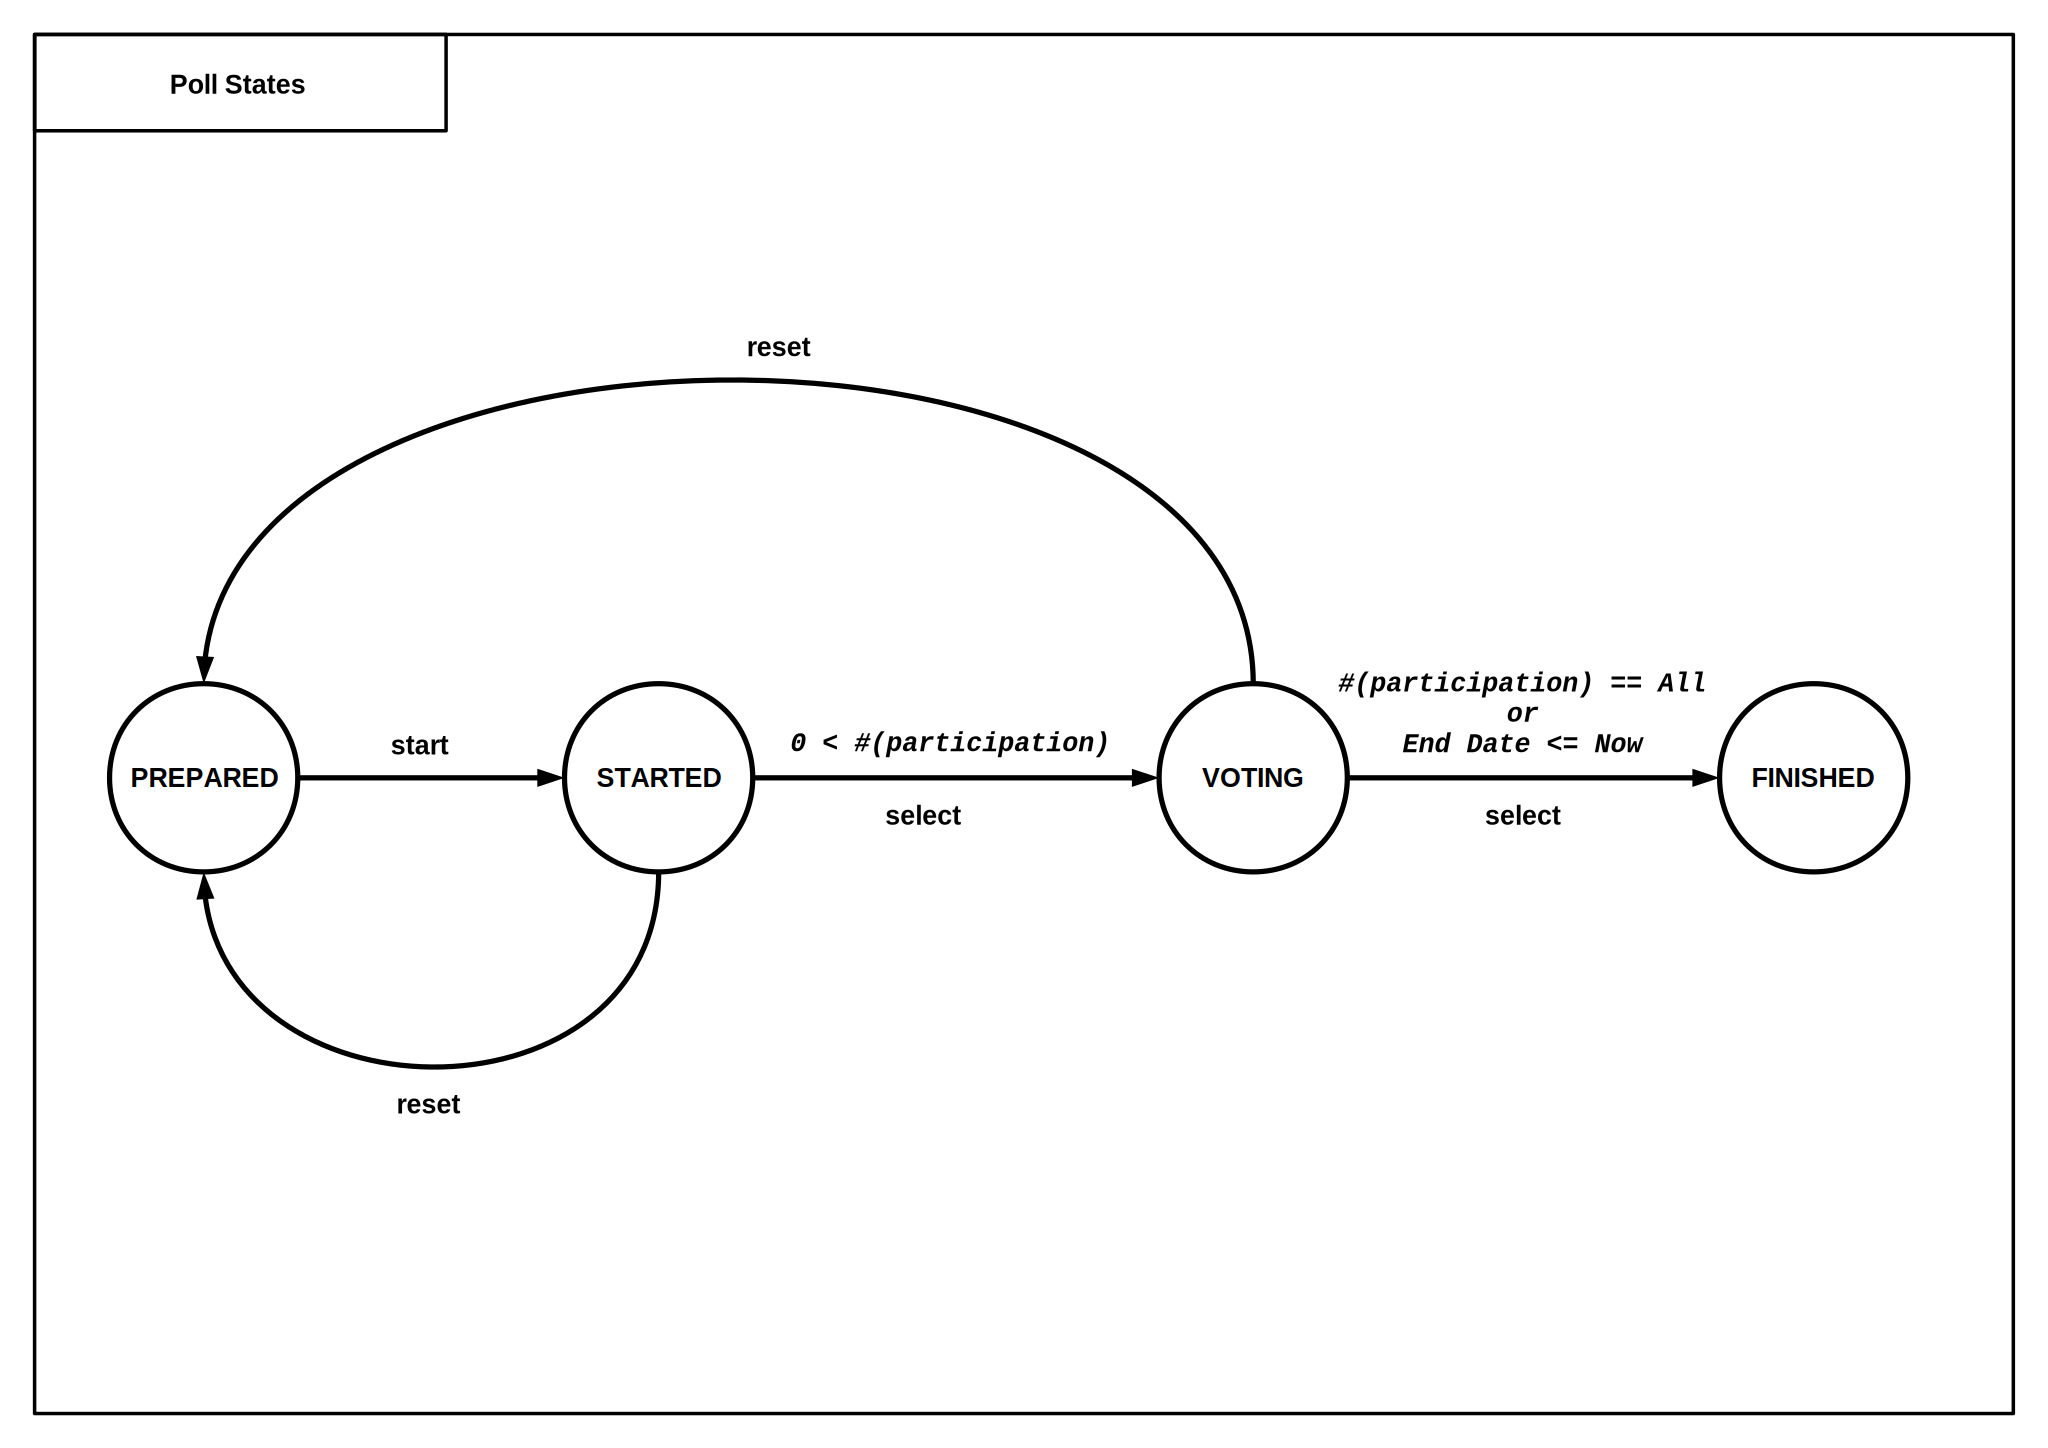
\includegraphics[width=0.9\textwidth]{png/poll-states.png}
\caption{Poll States}
\end{figure}
\section{Architecture}
% Follow UWE? Mabye good? I tink it maches not baad in this case. http://uwe.pst.ifi.lmu.de/teachingTutorial.html

\begin{figure}
\centering
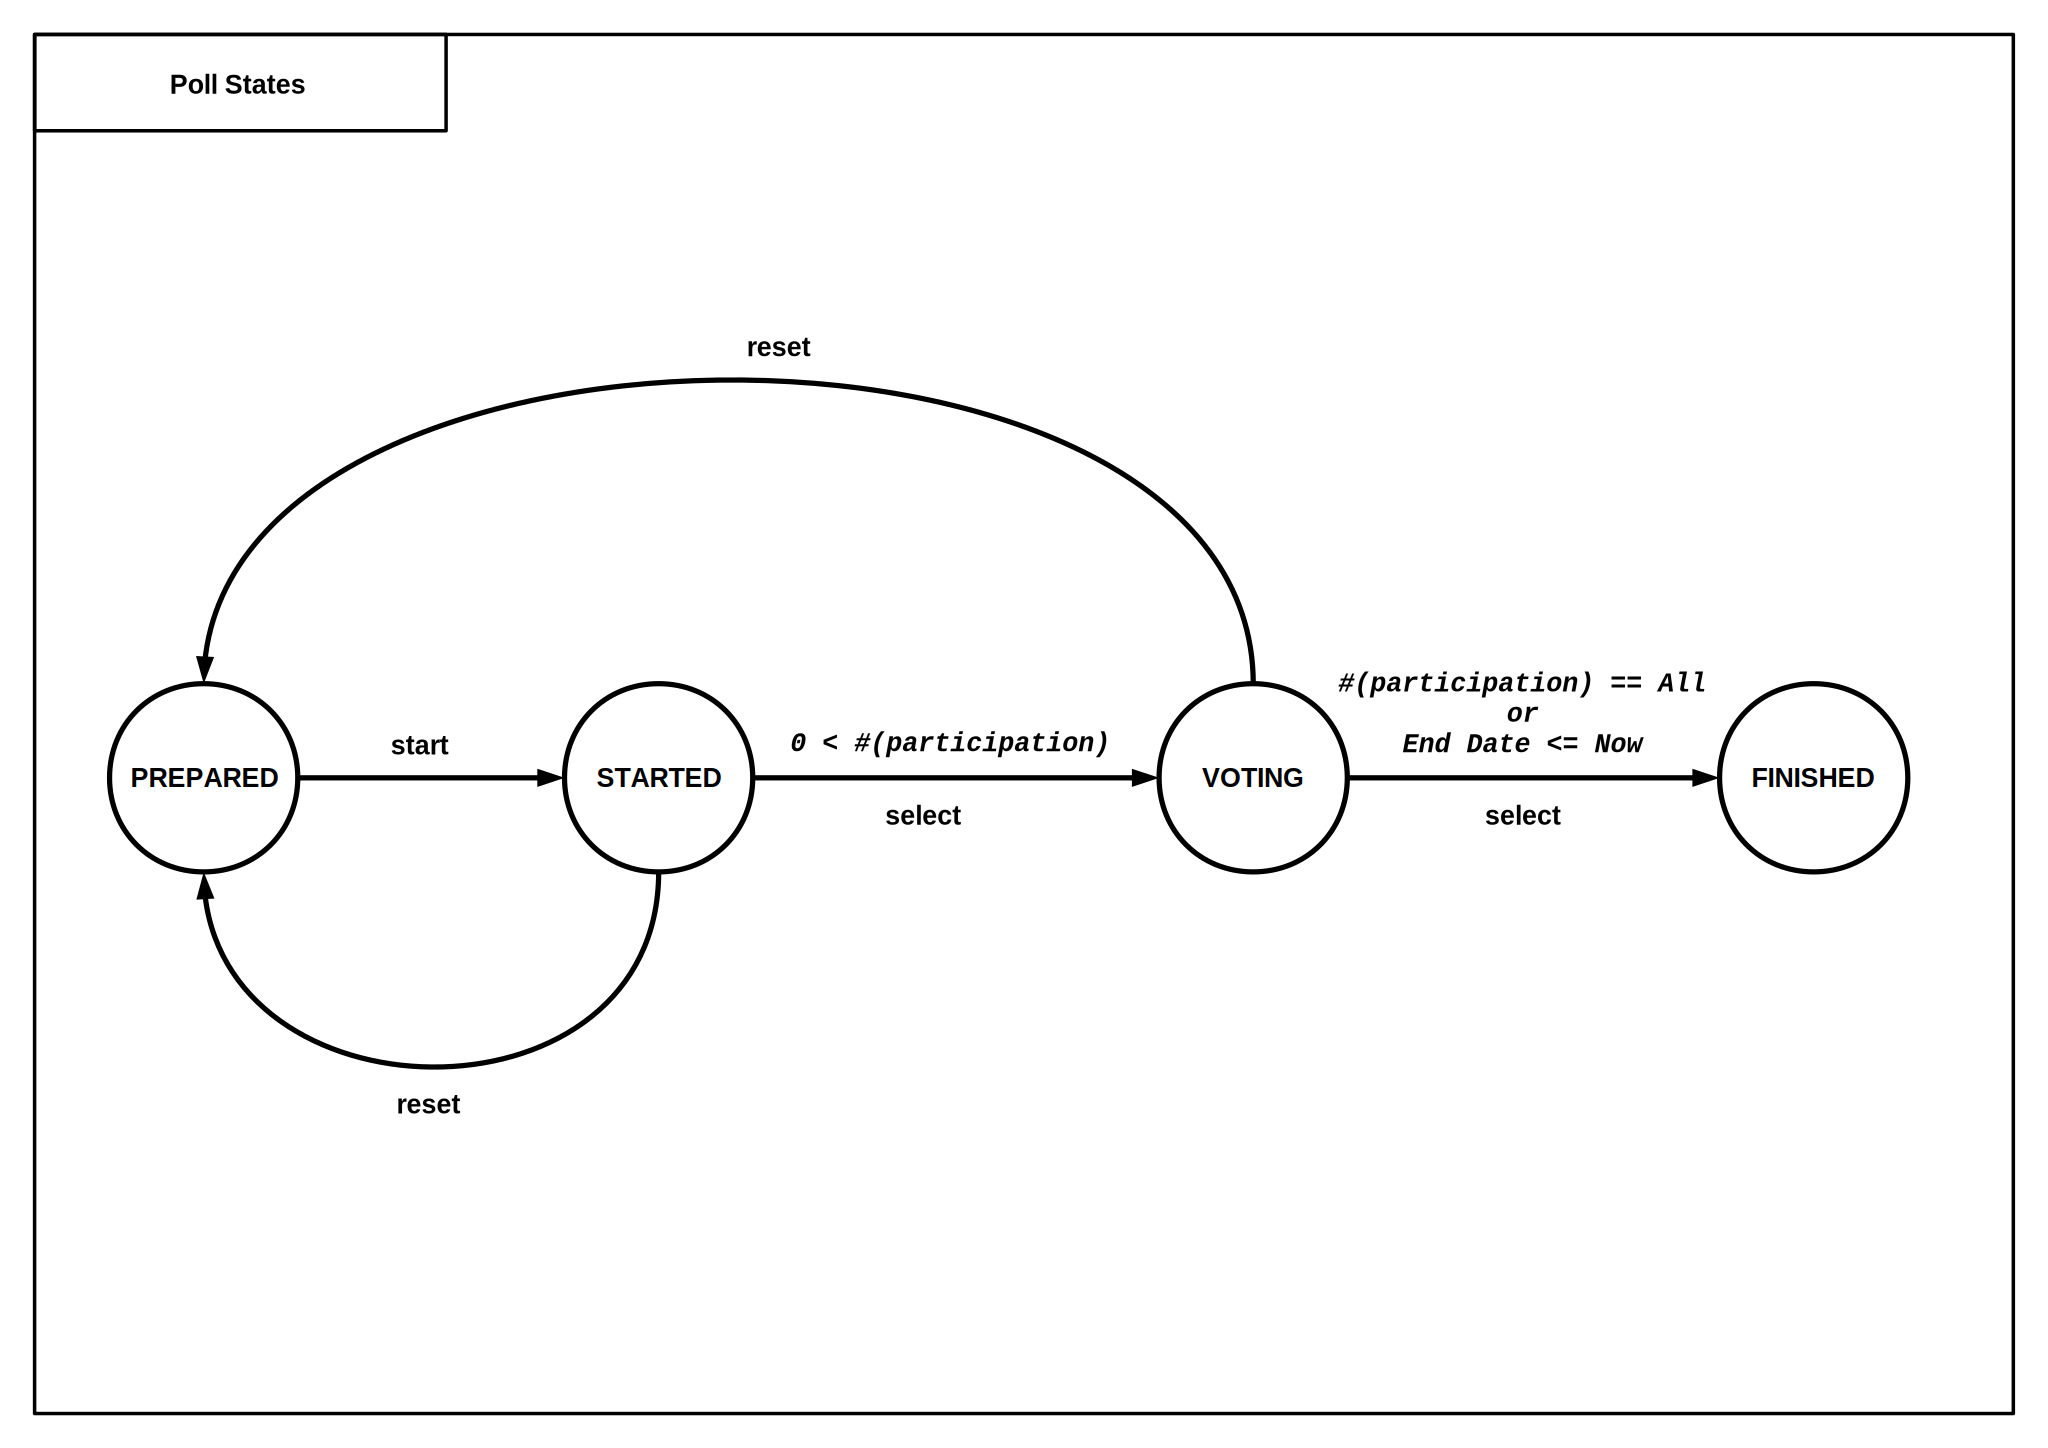
\includegraphics[width=0.9\textwidth]{png/poll-states.png}
\caption{Poll States}
\end{figure}

\subsection{Content Model}
The following view describes the systems content model. The corresponding implementation serves as backbone of the running application in form of keeping the data and persisting it. In the case of the content model, no presentation concerns are included. As well as that no behaviour is defined here. The six classes represent all essential entity types that are involved in the requirements. Two enumeration types serve as additional datatypes. 

High value comes to this view due to the fact that it can be directly be mapped on the JPA and the transfer object classes contained in the systems implementation. Apart from the fixed nature of the content model, described in the current requirements, a derivation process defining the Java classes can be of high good for further evolution and maintenance of the deployed system providing constitutive quality assurance.

\begin{figure}
\centering
\includegraphics[width=1.0\textwidth]{png/domain_model.png}
\caption{Votes content model}
\end{figure}


\subsection{VotesEJB Architecture}
% Maybe we can call that navigation model? Enables refference on http://uwe.pst.ifi.lmu.de/teachingTutorialNavigation.html
%Mentioned by ebert in the last web engeneering course! Will make rudige cum!
\subsection{VotesWar Architecture}
% Do you mean packaging?
\appendix
\section{Installation Guide}
\subsection{Database Installation}
\subsubsection{Connection Pool}
\subsubsection{JDBC Resource}
\subsection{Mail Session}
%\section{Manual}
In the following section the most important functionalities of the votes system are summarized.

\subsection{Login}

The Votes login page displayed in figure \ref{F:votes_login} is the entry-point to the system. A direct login is possible by entering an already registered email address an the correct password to the account. If no account has been created the user can sign in by first select \textit{Register} in the menu appearing when clicking on the top right button. If the resolution of the browser is high the menu is replaced by buttons in the black top bar. Clicking the \textit{Register} button is followed by the registration page. A valid account requires a \textit{Username}, \textit{Realname}, \textit{Email} and \textit{Password}.

\begin{figure}
\centering
\includegraphics[width=0.4\textwidth]{png/votes_login.png}
\caption{Votes login page}
\label{F:votes_login}
\end{figure}

\subsection{Browse my Polls}
When logged in the \textit{My Polls} page, displayed in figure \ref{F:browse_my_polls}, appears. Here all \textit{Polls} and some poll properties can be viewed on one single page. For informations that go deeper into the \textit{Polls} data the \textit{Poll} has to be clicked. The table displays title, state and results. The results can only be viewed when available.

\begin{figure}
\centering
\includegraphics[width=0.5\textwidth]{png/browse_my_polls.png}
\caption{Top part of the Votes \textit{Edit Poll} page}
\label{F:browse_my_polls}
\end{figure}



\subsection{Create and edit Polls}

\textit{Polls} can be created by pressing the \textit{New Poll} button that is located on the upper left corner of every page. By pressing \textit{New Poll} the user gets to a form were an initial \textit{Title} and \textit{Description} have to be entered. After that the user gets to the \textit{Edit Poll} page that can also be entered form the \textit{My Polls} page when selecting an existing poll.

\begin{figure}
\centering
\includegraphics[width=0.5\textwidth]{png/edit_poll.png}
\caption{Upper part of the Votes 'Edit Poll' page}
\label{F:edit_poll}
\end{figure}

The first part of the \textit{Edit Poll} page can be seen in figure \ref{F:edit_poll}. In this case it shows the concrete Poll with the title 'Java EE'. In the four text fields the \textit{Title}, \textit{Description}, \textit{End-Date} and \textit{Notification-Text} can be set. If \textit{Save} is pressed the setting are stored. The \textit{Delete} button deletes the poll. The appearance of the buttons \textit{Reset} and \textit{Start} are dependent on the state of current \textit{Poll}. In figure \ref{F:edit_poll} the \textit{Poll} has the state \textit{Started}, displayed next to the current \textit{Title} in the heading. In this case only the \textit{Reset} button is displayed.  

\begin{figure}
\centering
\includegraphics[width=0.5\textwidth]{png/items.png}
\caption{Middle part of the Votes \textit{Edit Poll} page displaying the items of the corresponding poll}
\label{F:items}
\end{figure}

In the middle part of the \textit{Edit Poll} page the list of \textit{Items} belonging to this \textit{Poll} can be edited. This is shown in figure \ref*{F:items}. If the \textit{Poll} is not already in the state \textit{Started}, the user has the option to add an \textit{Item} to the list by pressing the \textit{Add Item} button. The \textit{Title} and \textit{Type} fields are used for the creation of the new \textit{Item}. The possible Types are \textit{YES NO},\textit{ONE OF N} and \textit{M OF N}. All \textit{Items} can be opened by clicking on them in order to modify the \textit{Options}, the \textit{Title} or the \textit{Type}. The opportunity the add, remove or modify \textit{Options} is only given for the \textit{Items} of the \textit{Type} \textit{ONE OF N} and \textit{M OF N}.

\begin{figure}
\centering
\includegraphics[width=0.5\textwidth]{png/participants.png}
\caption{Bottom part of the Votes \textit{Edit Poll} page displaying the participants of the \textit{Poll}}
\label{F:participants}
\end{figure}

In the bottom part of the \textit{Edit Poll} page, displayed in figure \ref*{F:participants}, participants can be added and removed for the current poll. This is done by writing all mail addresses into the text field and pressing the \textit{Add Participants} button. When the Poll is started the all persons in the list are informed.

\subsection{Vote by using a Token}

\begin{figure}
\centering
\includegraphics[width=0.5\textwidth]{png/token.png}
\caption{Page for entering \textit{Tokens}}
\label{F:token}
\end{figure}

To vote in the system the \textit{Token} that has been sent by mail must be entered into the page displayed in \ref{F:token}. The link to this page is send ahead with the notification mail. If the \textit{Token} is correct the corresponding voting options appear by pressing the \textit{Verify} button.

% Bibliography
%%%%%%%%%%%%%%%%%%%%%%%%%%%%%%%%%%%%%%%%%%%%%%%%%%%%%%%%%%%
{
	\footnotesize
	\bibliography{handbook}
	\bibliographystyle{abbrv}
}

\end{document}